\begin{refsection}[research/ono/group.bib]
\nocite{*}
\chapter{Advanced Visualization Research Team}

\section{Members}

\begin{itemize}
  \item[] Kenji Ono (Team Leader)
  \item[] Jorji Nonaka (Researcher)
  \item[] Mikio Iizuka (Researcher)
  \item[] Chongke Bi (Postdoctoral Researcher)
  \item[] Daisuke Sakurai (Postdoctoral Researcher)
  \item[] Kazunori Mikami (Technical Staff)
  \item[] Tomohiro Kawanabe (Technical Staff)
  \item[] Seiji Fujino (Senior Visiting Scientist)
  \item[] Naohisa Sakamoto (Visiting Scientist)
  \item[] Masahiro Fujita (Visiting Technician)
  \item[] Kentaro Oku (Visiting Technician)
  \item[] Steve Petruzza (Student Trainee)
  \item[] Yukiko Hayakawa (Assistant)
  \item[] Keiko Matsuoka (Assistant)
\end{itemize}

\section{Research Activities}

Although the research activities of this team cover a broad range of the end-to-end simulation pipeline, including simulation, visualization and analysis, the main activities are centered on the study, design, and development of effective tools and mechanisms for visualization and analysis of large-scale parallel simulation results generated by the K computer. In this fiscal year, the team has worked on some core technologies necessary for building a production-level visualization and analysis framework. Taking into consideration the heterogeneous hardware infrastructure for post-processing, which includes the K computer itself, some post-processing servers, a visualization oriented GPU cluster, and local computer devices, we have worked on a framework named {\bf HIVE (Heterogeneously Integrated Visual analytics Environment)} \cite{2015:AVRTeam:HIVE}. Some of the core technologies, for enabling large data visualization and analysis, include a scalable parallel image compositing library for massively parallel rendering environments {\bf (234Compositor)} \cite{2015:Nonaka:JASSE, 2015:Nonaka:IPSJ-HPCS, 2015:Nonaka:HPCS}, a visual data analysis mechanism for multivariate data {\bf (Fiber Surface)}, a performance monitoring library for scientific applications {\bf (PMlib)} \cite{2015:AVRTeam:PMlib}, a multi-display management library for building scalable cooperative workspace on tiled wall displays {\bf (ChOWDER)} \cite{2015:AVRTeam:Chowder}, a parallel-in-time integration framework {\bf (PinT)} based on {\it Parareal} algorithm, and a sparse modeling approach based data compression for {\it in-situ} visualization {\bf (Sparse Modeling)}.

Effective visualization and analysis of large-scale data sets generated by modern leading-edge supercomputers such as the K computer is widely recognized as a difficult and challenging problem. There is still a lot of discussion among researchers about this topic, and we can cite the Dagstuhl-style {\it Shonan Meeting Seminar} focusing on {\it ``Big Data Visual Analytics''} \cite{Ono:2015:Shonan}, and also a panel discussion entitled {\it ``Top Computational Visualization R\&D Problems 2015''} \cite{Ono:2015:SA15} during the {\it Symposium on Visualization in High Performance Computing}. Our research activities have focused on a sustainable long-term development lifecycle for the HIVE framework, trying to assure the easiness for enhancement, maintenance and support, and also mechanisms for absorbing the heterogeneity of the computer platforms normally found on modern HPC operational environments. In addition to these items, we have also considered the following topics: easy usability; customizability for enabling diverse visualization scenarios; interactivity for finding the best visualization parameters; and in-situ processing mechanisms.

Most of the results of aforementioned research and developemnt efforts have already been released as open source libraries and applications, which are continuously maintained and updated. Following are the full list of those libraries and applications: {\it PDMlib}~\cite{2015:AVRTeam:PDMlib}; {\it UDMlib}~\cite{2015:AVRTeam:UDMlib}; {\it HDMlib}~\cite{2015:AVRTeam:HDMlib}; {\it CDMlib}~\cite{2015:AVRTeam:CDMlib}; {\it Polylib}~\cite{2015:AVRTeam:Polylib}; {\it Cutlib}~\cite{2015:AVRTeam:Cutlib}; {\it LPTlib}~\cite{2015:AVRTeam:LPTlib}; {\it TextParser}~\cite{2015:AVRTeam:TextParser}; and {\it JHPCN-DF}~\cite{2015:AVRTeam:JHPCN-DF}.

\section{Research Results and Achievements}

\subsection{Visual Analytics Framework (HIVE)}

We integrated some of the core technologies listed in the previous section, and developed a prototype of the HIVE framework focusing on the operational environment of the K computer. Considering the hardware heterogeneity of this environment, which includes the K computer itself, some post-processing servers, visualization oriented GPU cluster, and local computational devices, HIVE was designed to run on {\it SPARC64fx CPUs}, {\it x86 CPUs}, and {\it GPUs}. Figure~\localref{fig:HIVE} shows the Web-based  User Interface(UI) designed for accessing the HIVE functionalities, and for small data sets it is possible to execute the entire visualization and analysis on the local computational side. For larger data sizes, this Web-based UI can be useful for preparing the visualization scenes to be used as a parameter during the batch job execution of large-scale parallel visualization processing. As shown in the Figure~\localref{fig:HIVE}, HIVE adopted the sort-last parallel rendering approach, which requires the image compositing {\bf process} right after the parallel rendering stage. It is worth noting that the scalability target of both parallel processing modules were the full node of the K computer.

\begin{figure}[b]
  \centering{
  	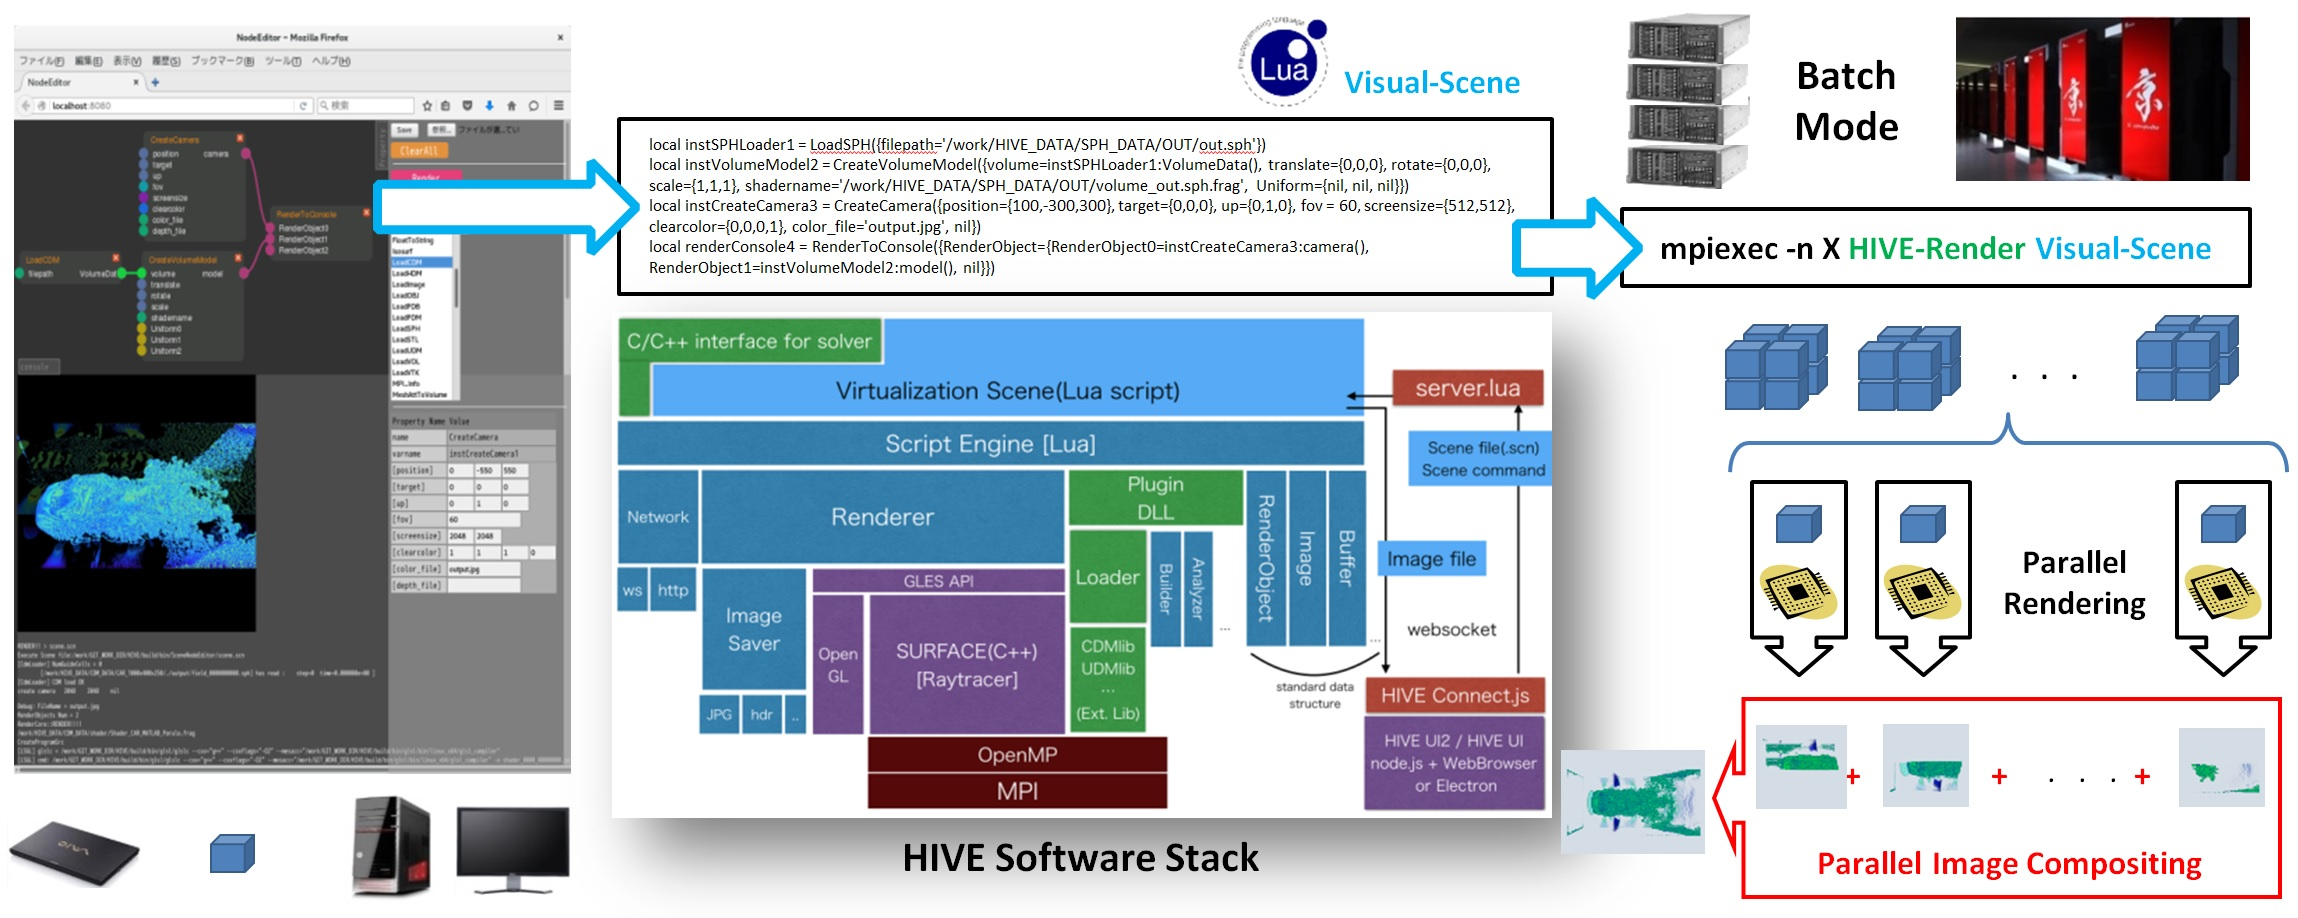
\includegraphics[width=0.99\textwidth]{research/ono/HIVE.jpg}
  }
  \caption{The software stack and the Web-based user interface of the HIVE framework designed for the visualization and analysis of large-scale simulation results generated from HPC platforms.}
  \locallabel{fig:HIVE}
\end{figure}

In order to enable the sustainable long-term development and maintenance life cycle of the HIVE framework, we focused on a minimum set of external libraries for avoiding the software dependency as much as possible. For instance, the {\bf SURFACE} rendering module adopted the {\it GLES 2.0} (OpenGL for Embedded Systems Version 2.0) compatible {\it API} (Application Programming Interface). The {\it GLES} is a subset of the original cross-language and multi-platform {\it OpenGL API} for rendering 2D and 3D vector graphics. This compatibility facilitates the development of both CPU and GPU based implementations. HIVE has designed to have a minimum but necessary set of functionalities, and the {\bf Plugin DLL} module facilitates the extensibility and maintainability of the HIVE system by separating the core modules and other external or third party modules. This feature is possible, in part, due to the adoption of the light-weight and multi-platform scripting language called {\bf Lua}. This scripting language is also used for describing the entire dataflow of a given visualization scene ({\bf Visual-Scene} in the Figure~\localref{fig:HIVE}), which can be easily converted to a batch job script for executing directly on the K computer. Examples of the third-party modules already incorporated to the HIVE include the large-scale parallel image compositing module {\bf (234Compositor)}, and a set of large-scale data management libraries {\bf (xDMlib)}. Other modules which are in the process of integration include those for visual analysis: {\bf (Fiber Surface)} and Performance Monitoring {\bf (PMlib)}.

\subsection{234Compositor}

\begin{figure}[b]
  \centering{
  	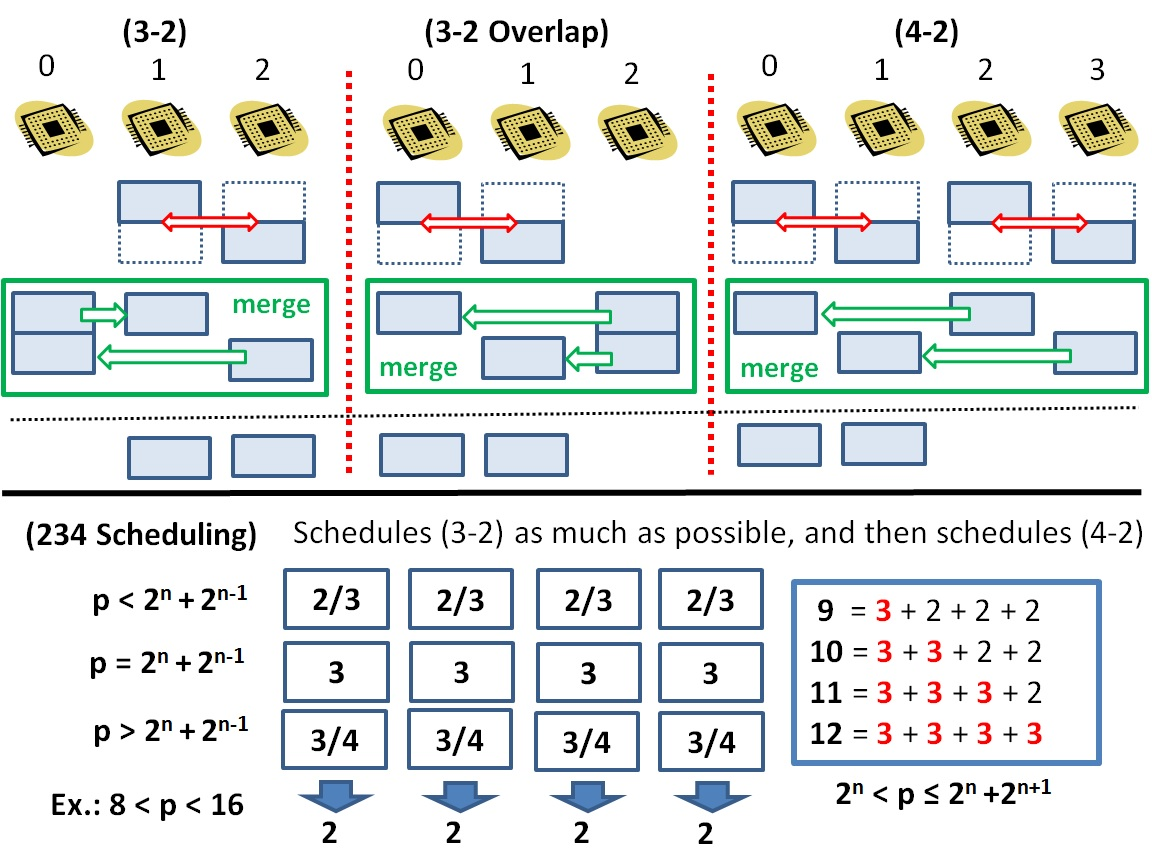
\includegraphics[width=0.47\textwidth]{research/ono/234_1.jpg}
 	\hspace{5mm}
  	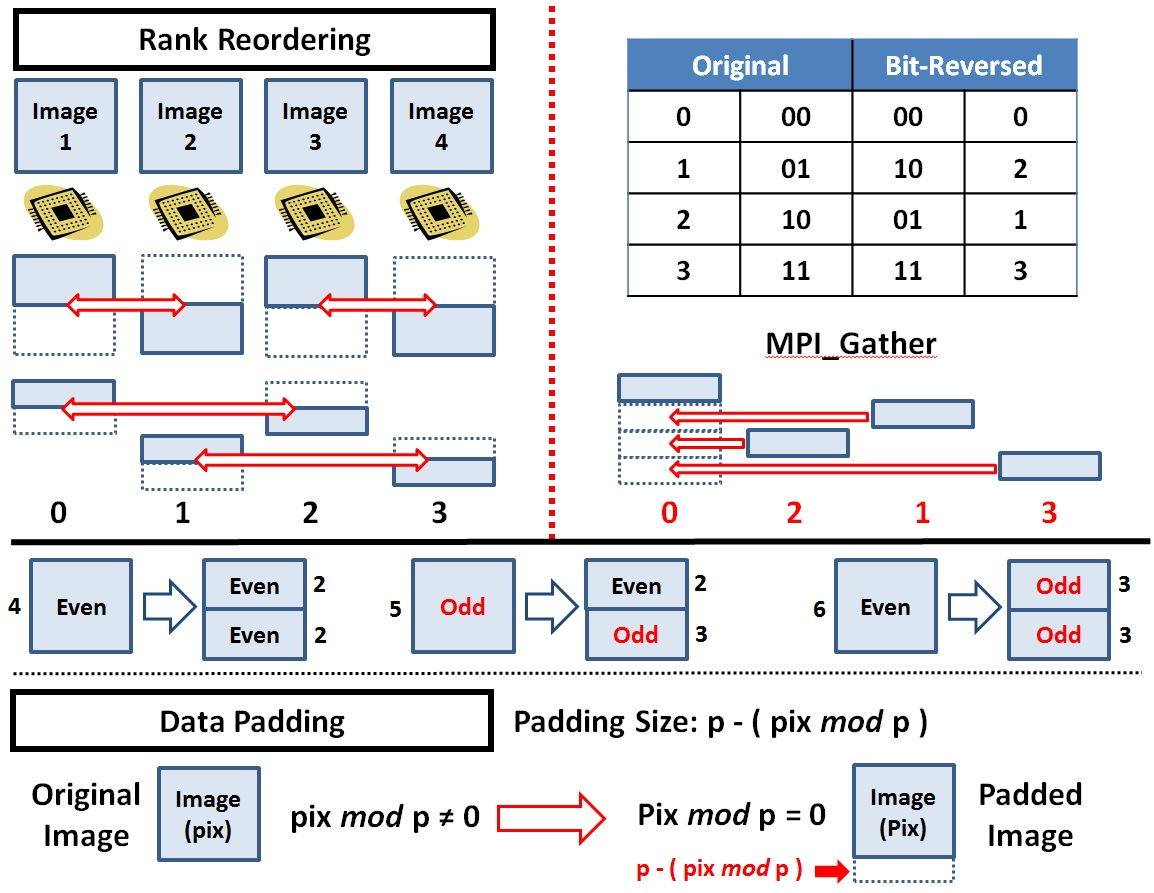
\includegraphics[width=0.47\textwidth]{research/ono/234_2.jpg}
  }
  \caption{{\it 3-2}, {\it 3-2 Overlap} and {\it 4-2 Eliminations} with the {\it 234 Scheduling} mechanism (Left side). {\it MPI Rank Reordering} and {\it Data Padding} for enabling the use of {\it MPI Gather} (Right side) }
  \locallabel{fig:234}
\end{figure}

The core rendering engine of the HIVE is a highly scalable {\it Raytracer} named {\bf SURFACE} (Scalable and Ubiquitous Rendering Framework for Advanced Computing Environments), which adopted the {\it Sort-last parallel rendering} approach, that is, after the parallel rendering stage the entire set of rendered images should be gathered and merged into the final single image as shown in the Figure~\localref{fig:HIVE}. To meet the performance and scalability demands of the SURFACE, we have developed the {\it 234Compositor}, a hybrid MPI/OpenMP parallel image compositor library, based on the well-known {\it Binary-Swap} parallel image compositing algorithm. Although Binary-Swap has proven highly scalable, there exist some issues including the requirements for power-of-two number of processes, and the final sub-image collecting cost by using the {\it MPI\_Gatherv} collective operation.

There already exist some extensions for the Binary-Swap to enable the use with non-power-of-two number of processes. One of these extensions is {\it Telescoping} method where the number of processes is gradually converted to the largest power-of-two number of processes, and was implemented on the {\it Ice-T} parallel image compositing library adopted by some parallel visualization applications such as {\it ParaView} and {\it VisIt}. Although it has proven efficient on specific supercomputer hardware architectures, we focused on a single-stage conversion approach to minimize the conversion overhead, and utilized the {\it 3-2} and {\it 2-1 Eliminations} techniques proposed by {\it Rabenseifner et al.} for MPI communications involving non-power-of-two odd number of processes. We extended the original algorithm for enabling the use to the even number of processes by applying the {\it 234 Scheduling}~\cite{2015:Nonaka:HPCS}, as shown in Figure~\localref{fig:234}. The communication pattern of the {\it 3-2 Elimination} was also extended to enable the overlapping of communication and computation.

The final stage of the Binary-Swap image compositing algorithm is the gathering of image fragments, distributes among the image compositing nodes, to the master node and the assembly of the final image. In order to minimize the performance degradation when using a large number of node counts, we developed the {\it Multi-Step Image Composition} approach\cite{2015:Nonaka:JASSE}, which works by recursively dividing the composition nodes into smaller groups with a pre-defined threshold. We also worked on {\it MPI rank reordering} and {\it image data padding} techniques for enabling the use of {\it MPI\_Gather}, in substitution to the traditional {\it MPI\_Gatherv}, for optimizing the final image gathering stage\cite{2015:Nonaka:IPSJ-HPCS}. Figure~\localref{fig:234_82K} shows the performance evaluation results of the {\it 234Compositor}, which integrates the aforementioned techniques, and we could confirm the scalability up to the full node of the K computer when compositing 128-bit RGBA images with sizes varying from 1 to 32 MP (Mega Pixels).

\begin{figure}[tb]
  \centering{
  	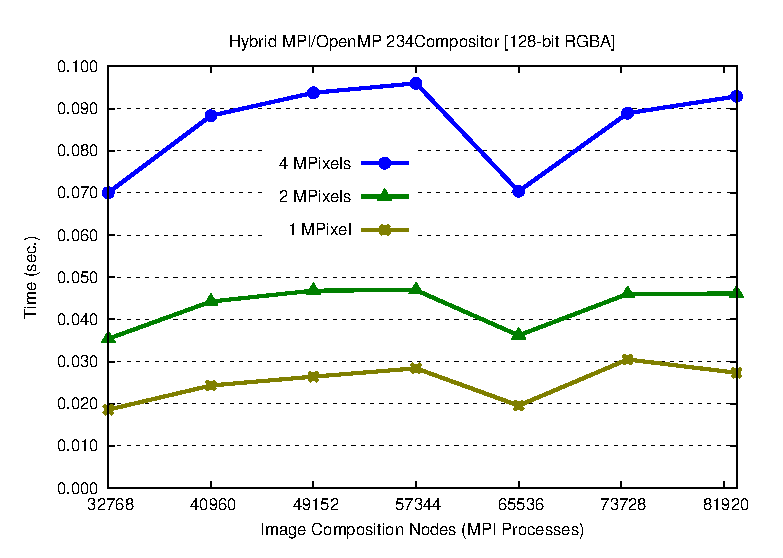
\includegraphics[width=0.47\textwidth]{research/ono/82k_gather_omp8_1-4.eps}
 	\hspace{5mm}
  	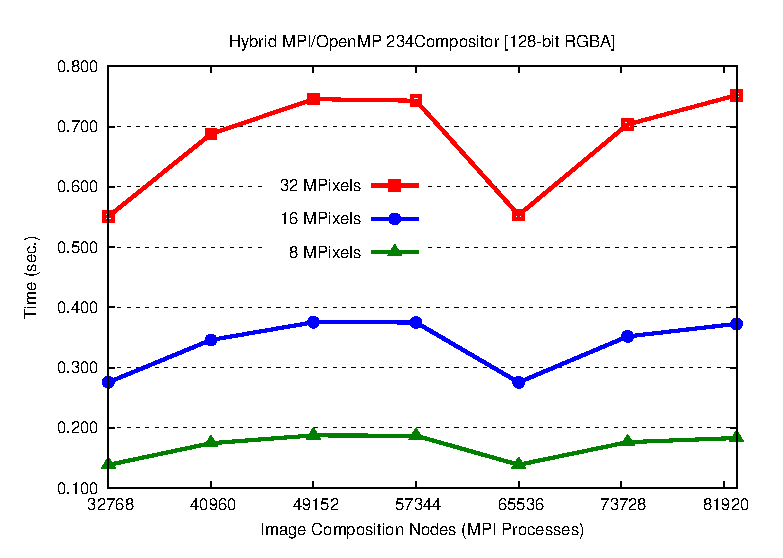
\includegraphics[width=0.47\textwidth]{research/ono/82k_gather_omp8_8-32.eps}
  }
  \caption{Scalability evaluation of the {\it 234Compositor} for image sizes from 1 to 32 Mega Pixels (RGBA 128-bit) using up to the full node of the K computer.}
  \locallabel{fig:234_82K}
\end{figure}

\subsection{Fiber Surface}

With our \emph{fiber surface GUI} (Fig. \localref{fig:fibersurface-ds}), a user can analyze multivariate data to quickly extract 3D features such as vortex structures in meteorology data and objects in CT scans. When the user is familiar with the popular isosurface analysis, it is not difficult to understand the concept of fiber surface -- it is a straight-forward generalization of isosurface.
The GUI is integrated into HIVE so that the user can analyze large-scale datasets in various computational architectures. In fact, multivariate datasets are often the output of simulations in supercomputers like the K computer.
The user explores data by querying data values of interest. The query is as simple as drawing a polygon in a scatterplot. Our GUI then visualizes the queried samples in the 3D coordinate as 2D polyhedra. Thanks to fiber surface, the data size becomes magnitudes smaller compared to the original 3D data. This means that once the fiber surface is extracted, even computers with weaker performance can visualize the simulation outputs efficiently. The GUI resembles to traditional isosurfacing tools, while respecting today's GUI design for multifield exploration. The GUI also offers a scripting environment in order to support flexible data analysis.

\begin{figure}[h]
  \centering{
%  	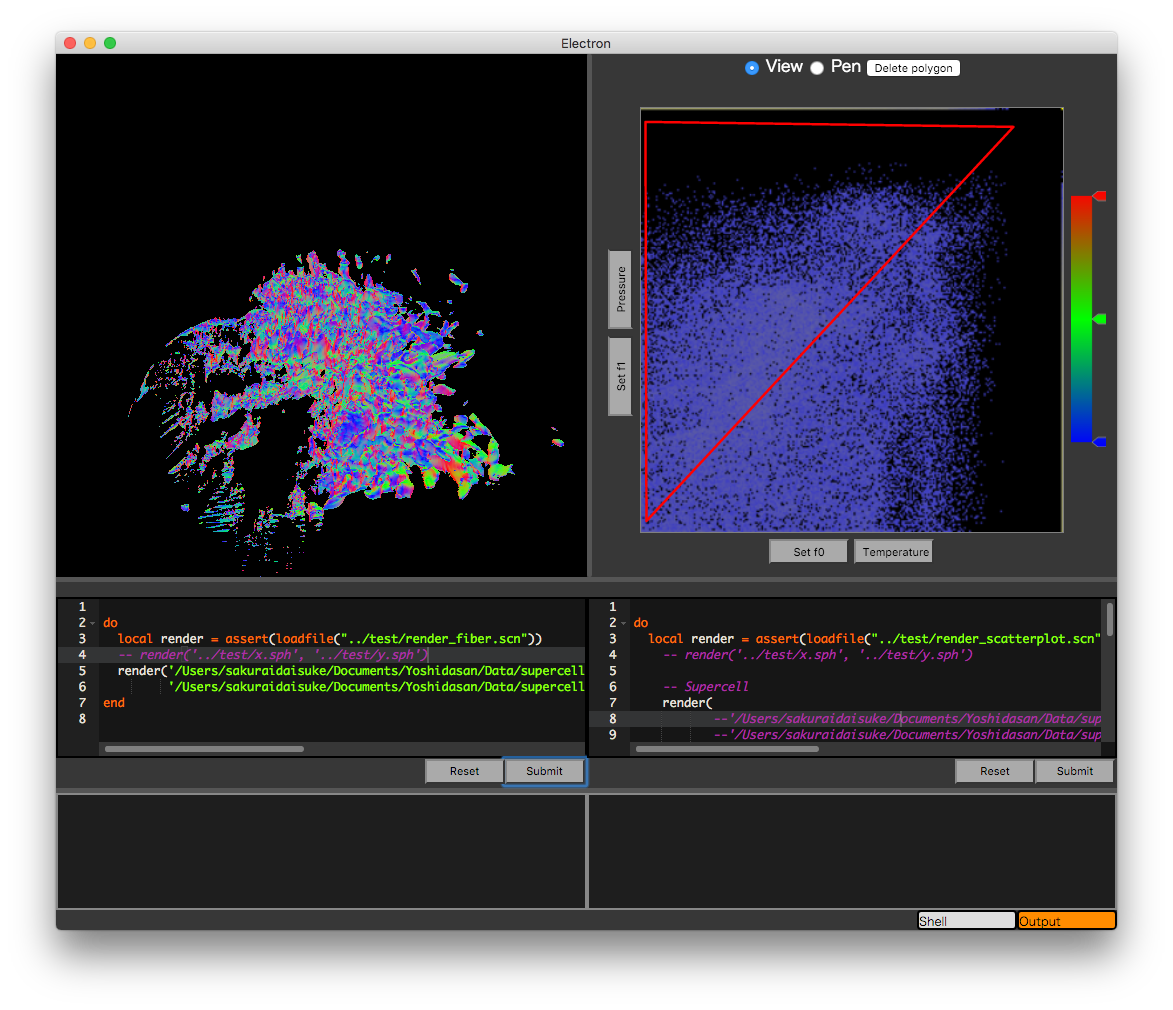
\includegraphics[width=0.8\hsize]{research/ono/fibersurface-ds.png}
  	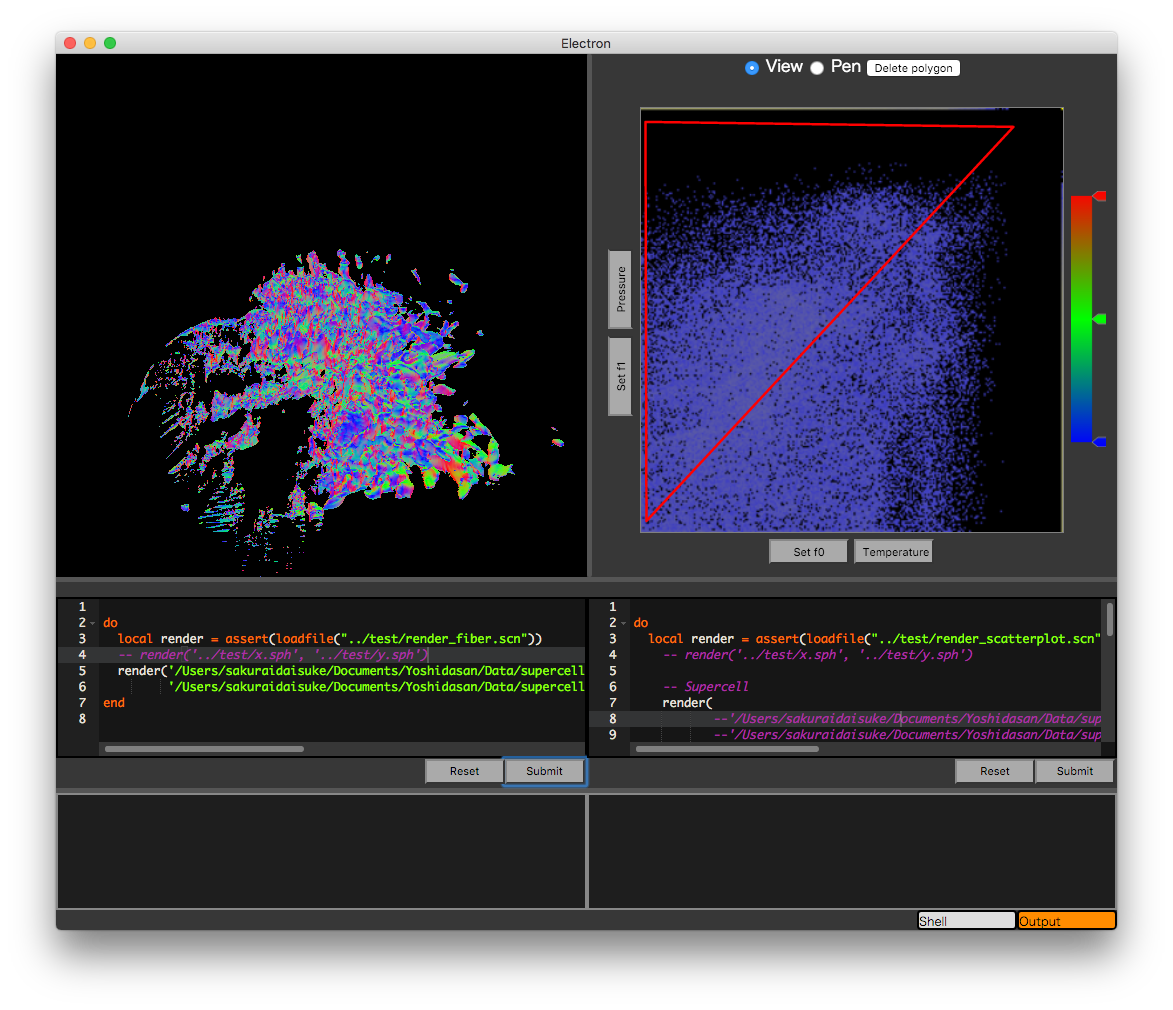
\includegraphics[height=0.35\textheight]{research/ono/fibersurface-ds.png}
  }
  \caption{Fiber surface GUI visualizing water cohesion in the atmosphere (simulated with SCALE, which is developed by the Computational Climate Science Research Team of RIKEN AICS).}
  \locallabel{fig:fibersurface-ds}
\end{figure}

\subsection{Development of PMlib (Performance Monitoring Library)}

PMlib is an open source software library designed for monitoring the computational performance of scientific applications. PMlib has designed to support hybrid parallelism where the parallel distributed memory and shared memory computing are exploited by the applications through specific libraries such as MPI and OpenMP. This library is suitable for monitoring computational workloads of applications which can change dynamically over the time and space, depending on their initial conditions and state variables, such as computing particle trajectories over the subdomains in parallel fluid simulations.

The performance statistics for the computational workload such as floating point operations per second (flops) and memory load/store operations per second (bandwidth) can either be defined as the algorithmic workload, that is, theoretical requirements decided by the source program, or as the actually executed system workload. The latter varies depending on the system conditions including the compiler optimization, prefetch strategy and data movement on hierarchical cache components, and numbers of pipeline stages for arithmetic operations. 

This library allows the users to select the best policies to obtain the statistics during runtime executions. The statistics policies can be explicitly declared by the users as API arguments inside the source program, or can be automatically acquired from the processor built-in hardware counters. PMlib will produce the report in text format at a post processing phase as shown in Figure~\localref{fig:mikami-fig1}.

%Some example PMlib output results are shown below.
%\begin{figure}[H]
\begin{figure}[htb]
%\begin{tabular}{cc}
\begin{minipage}{0.5\hsize}
\centering
%\tiny
\scriptsize
%\footnotesize
\begin{verbatim}
Parallel Mode:   Hybrid (8 processes x 2 threads)
The environment variable HWPC_CHOOSER=FLOPS is provided.
Total execution time            = 2.270602e+00 [sec]
Exclusive sections statistics per process and total job.
Inclusive sections are marked with (*)

Section           |call|        accumulated time[sec]          | [hardware counter flop counts]
Label             |    |      avr   avr[%]      sdv   avr/call |      avr       sdv   speed
------------------+----+---------------------------------------+----------------------------
First section     :   1  9.086e-01  30.29  5.52e-01  9.086e-01   5.909e+09  7.25e+08   6.50 Gflops
Second section(*) :   1  1.996e+00  66.54  4.18e-01  1.996e+00   5.752e+09  3.94e+08   2.88 Gflops(*)
Subsection X      :   1  7.349e-01  24.50  1.89e-01  7.349e-01   6.586e+09  5.32e+08   8.96 Gflops
Subsection Y      :   1  6.123e-01  20.41  1.26e-01  6.123e-01   5.896e+09  3.49e+08   9.63 Gflops
------------------+----+---------------------------------------+----------------------------
Sections per process     2.256e+00    -Exclusive CALC sections-  1.839e+10             8.15 Gflops
------------------+----+---------------------------------------+----------------------------
Sections total job       2.256e+00    -Exclusive CALC sections-  1.471e+11            65.22 Gflops
\end{verbatim}
\end{minipage}
\caption{Output example of PMlib.}
\locallabel{fig:mikami-fig1}
\end{figure}

\begin{figure}[h]
  \centering{
  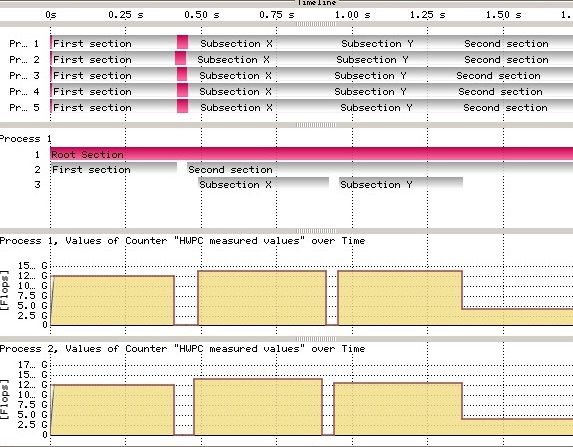
\includegraphics[width=100.0mm,keepaspectratio]{research/ono/mikami-fig2.jpg}
  }
  \locallabel{fig:mikami-fig2}
  \caption{Statistical view of PMlib's output.}
\end{figure}

\pagebreak
In this fiscal year, the development efforts for PMlib was focused on the following items:

\begin{itemize}
  %	\setlength{\itemsep}{-1.5mm}
  \setlength{\parskip}{-1.5mm}
  \item Fortran API support
  \item Multiple MPI group support
  \item Addition of example programs and update of the user document
  \item Addition of an optional sorted output
  \item Initial study of a graphical interface for the Open Trace Format
\end{itemize}

\subsection{ChOWDER}

\emph{ChOWDER} (\emph{\underline{Co}operative \underline{W}orkspace \underline{D}riv\underline{er}}) is a Web browser based multi-monitor controller system designed to assist collaborative work among multiple users and applications. The development of \emph{ChOWDER} has been conducted by the financial support of a cross-ministerial Strategic Innovation promotion Program (SIP) grant. \emph{ChOWDER} delivers the functionality of virtual display driver for tiled wall display, and can be used for building scalable cooperative workspace environment for designers and engineers.

As shown in Figure~\localref{fig:chowder}, \emph{ChOWDER} system is composed of the following three subsystems:

\begin{itemize}
  \setlength{\parskip}{-1.5mm}
  \item Client Controller
  \item Client Display
  \item Display Server
\end{itemize}

\begin{figure}[h]
   \centering{
   	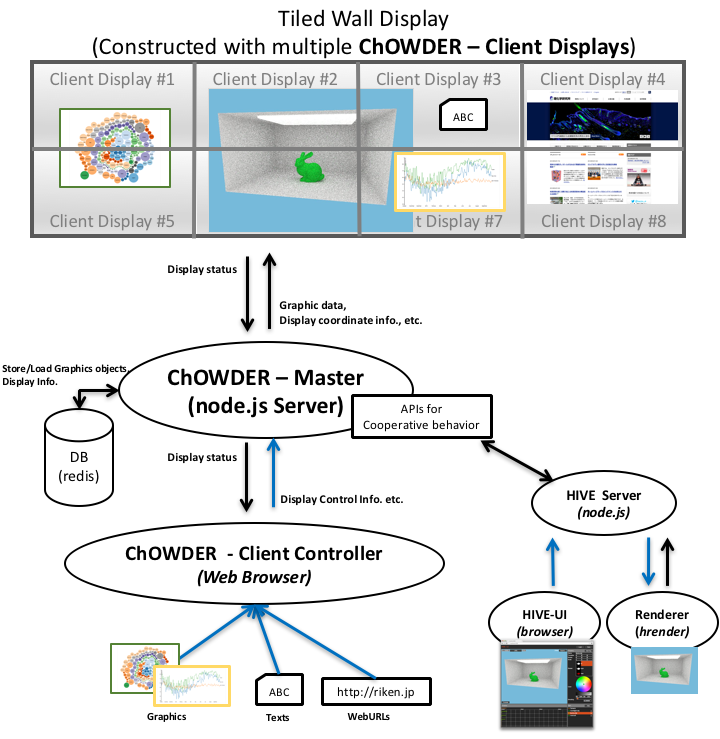
\includegraphics[height=0.4\textheight]{research/ono/chowder_diagram.png}
   }
   \caption{System diagram of ChOWDER.
   }
   \locallabel{fig:chowder}
\end{figure}

{\it Client Controller} is used for positioning the client displays on the user defined virtual display space. The controller is also used for positioning the displaying objects inside the virtual display space, via Web-based User Interface (UI) since {\it Client Controller} works inside the Web browser.

{\it Client Displays} are the physical displays where the contents in the virtual display space are actually displayed. Figure~\localref{fig:chowder} shows an example of 8 {\it Client Displays} forming a single virtual display, and the user can make a huge virtual display space by simply adding new {\it Client Displays} to these existing {\it Client Displays}. These subsystems can work on a variety of devices based on the following Operational Systems: Windows, Mac, Linux, iOS, and Android.
{\it Display Server} controls the communications between {\it Client Controller} and {\it Client Displays}, and manages the display objects to be displayed on {\it Client Displays}.
{\it Display Server} was implemented by using the {\it node.js}, {\it socket.io}, {\it websockets}, and {\it redis} technologies. As shown in the Figure~\localref{fig:chowder}, {\it Display Server} possesses an API for cooperative behavior, which enables a seamless communication with HIVE system, that is, the graphics output of the HIVE can be sent to \emph{ChOWDER's} {\it Client Displays}.


\subsection{Parallel-in-Time Integration}
%
\emph{Parallel-in-time integration (PinT)} is desired for effectively exploiting the concurrency of the post peta-scale parallel computing environments which are expected to increase the currently achievable degree of concurrency.
%
The study of PinT advances rapidly after \emph{the Parareal method}(Fig. \ref{fig:PinT-Framework}(a)) was proposed by Lions at the beginning of the 2000's.
%
The Parareal method has the characteristic that it is easy to reuse existing codes and it doesn't demand large memory capacity.
In other words, Parareal method provides us a general and practical framework to describe parallel-in-time integration algorithms for a variety of simulation codes.
Therefore, we have investigated a general-purpose PinT framework, which employs the {\it Parareal} method, to reduce the developer efforts for describing the PinT codes (Fig. \ref{fig:PinT-Framework}(b)).

We have investigated and found that {\it Parareal} method works well for parabolic PDEs, but does not work so well for hyperbolic PDEs. Therefore, we performed some investigations on the trends and prospects of PinT methods, and then we set a research direction for the PinT study.
As the next steps, we will intensively study the Reduced basis methods (Fig. \ref{fig:Methods}(a)) which use the sparse modeling technique, phase alignment methods (Fig. \ref{fig:Methods}(b)), adjoint-based methods which use symmetrization of the time-integrator and Parareal/SDC hybrid methods.
%
\begin{figure}[h]
    \begin{center}
    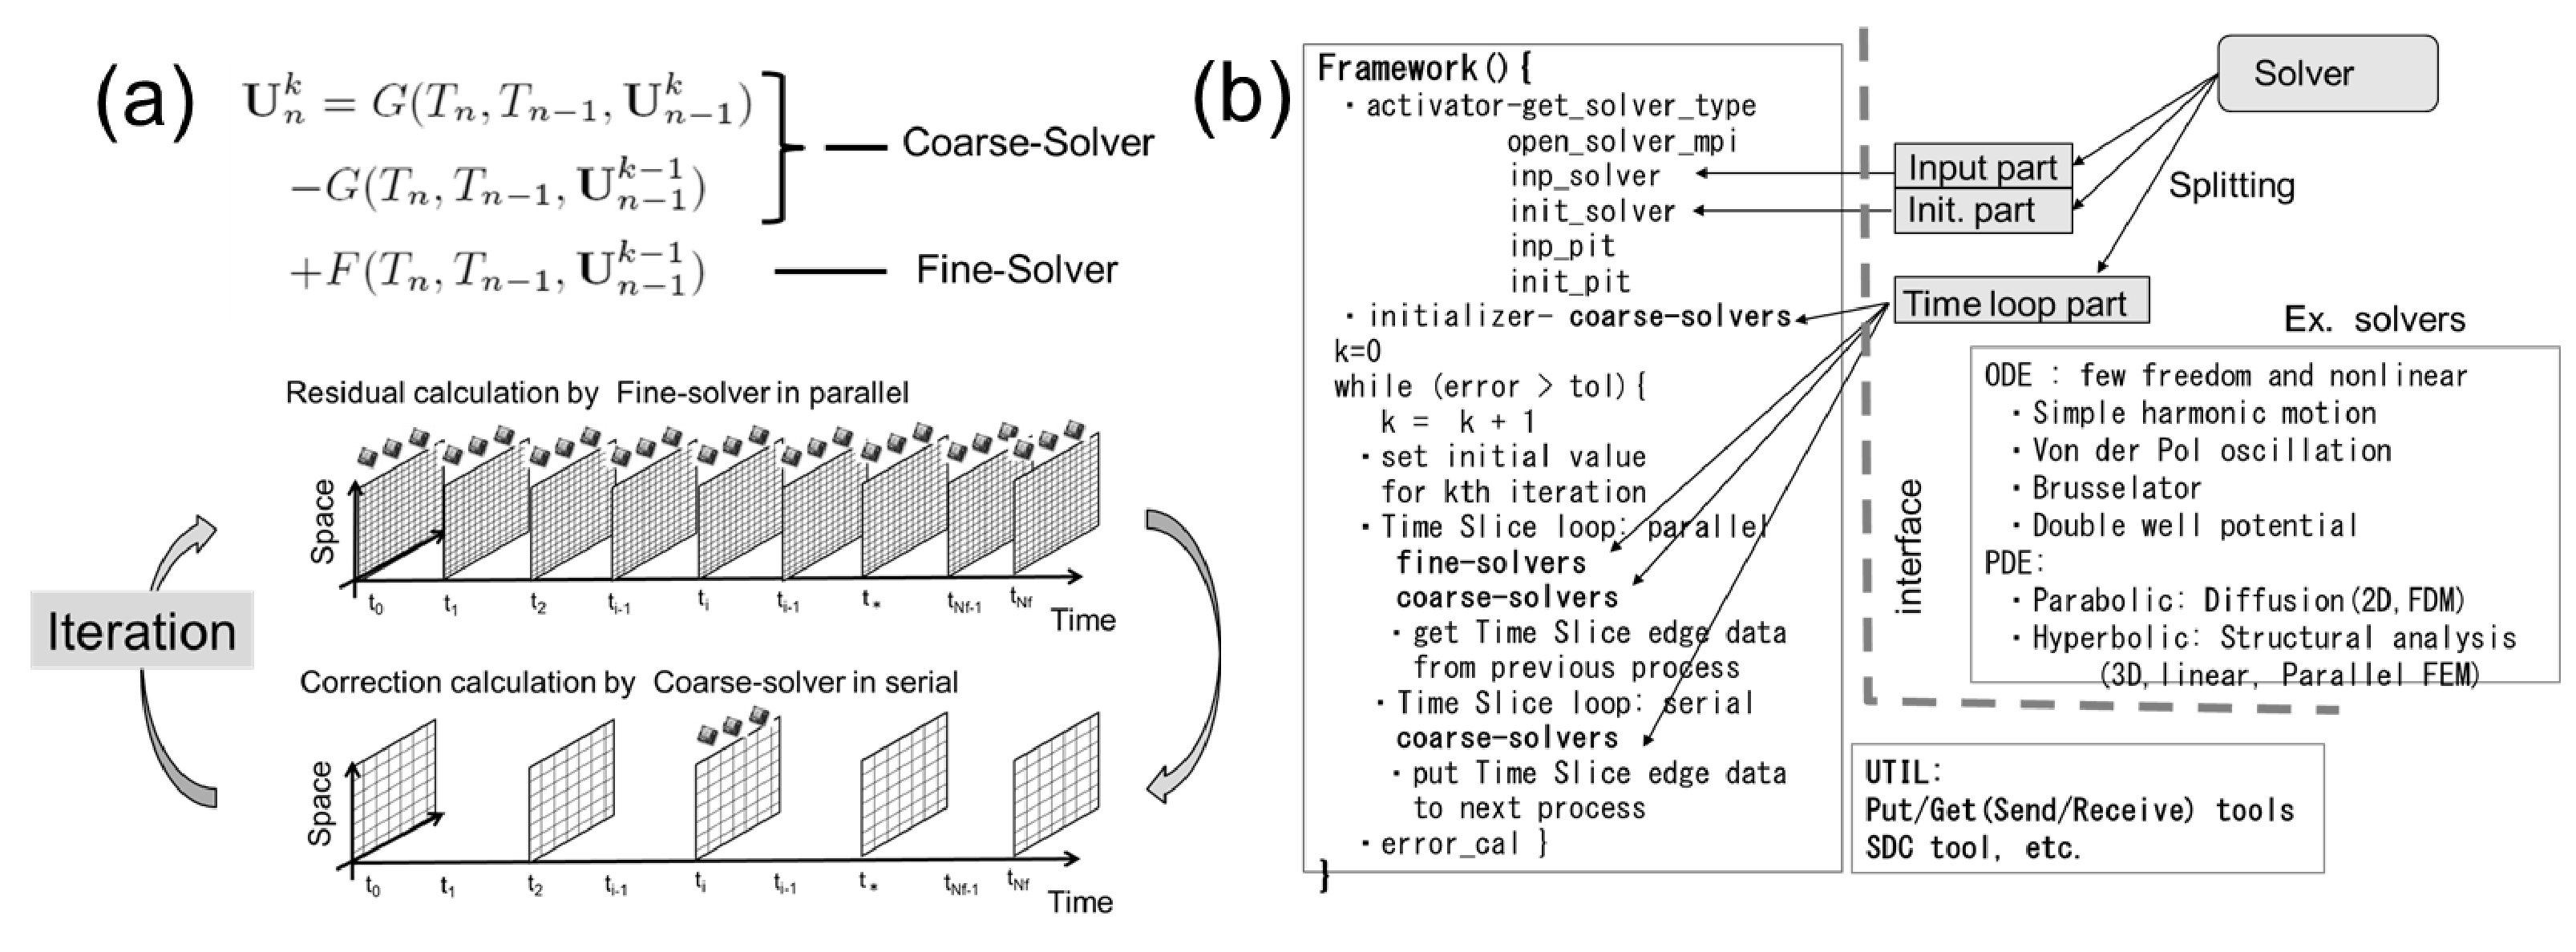
\includegraphics[scale=0.275]{research/ono/PinT-Framework.eps}
    \end{center}
    \caption{{\it PinT} framework: (a) {\it Parareal} algorithm, (b) Prototype of a {\it PinT} framework.}
    \label{fig:PinT-Framework}
\end{figure}

\begin{figure}[h]
    \begin{center}
    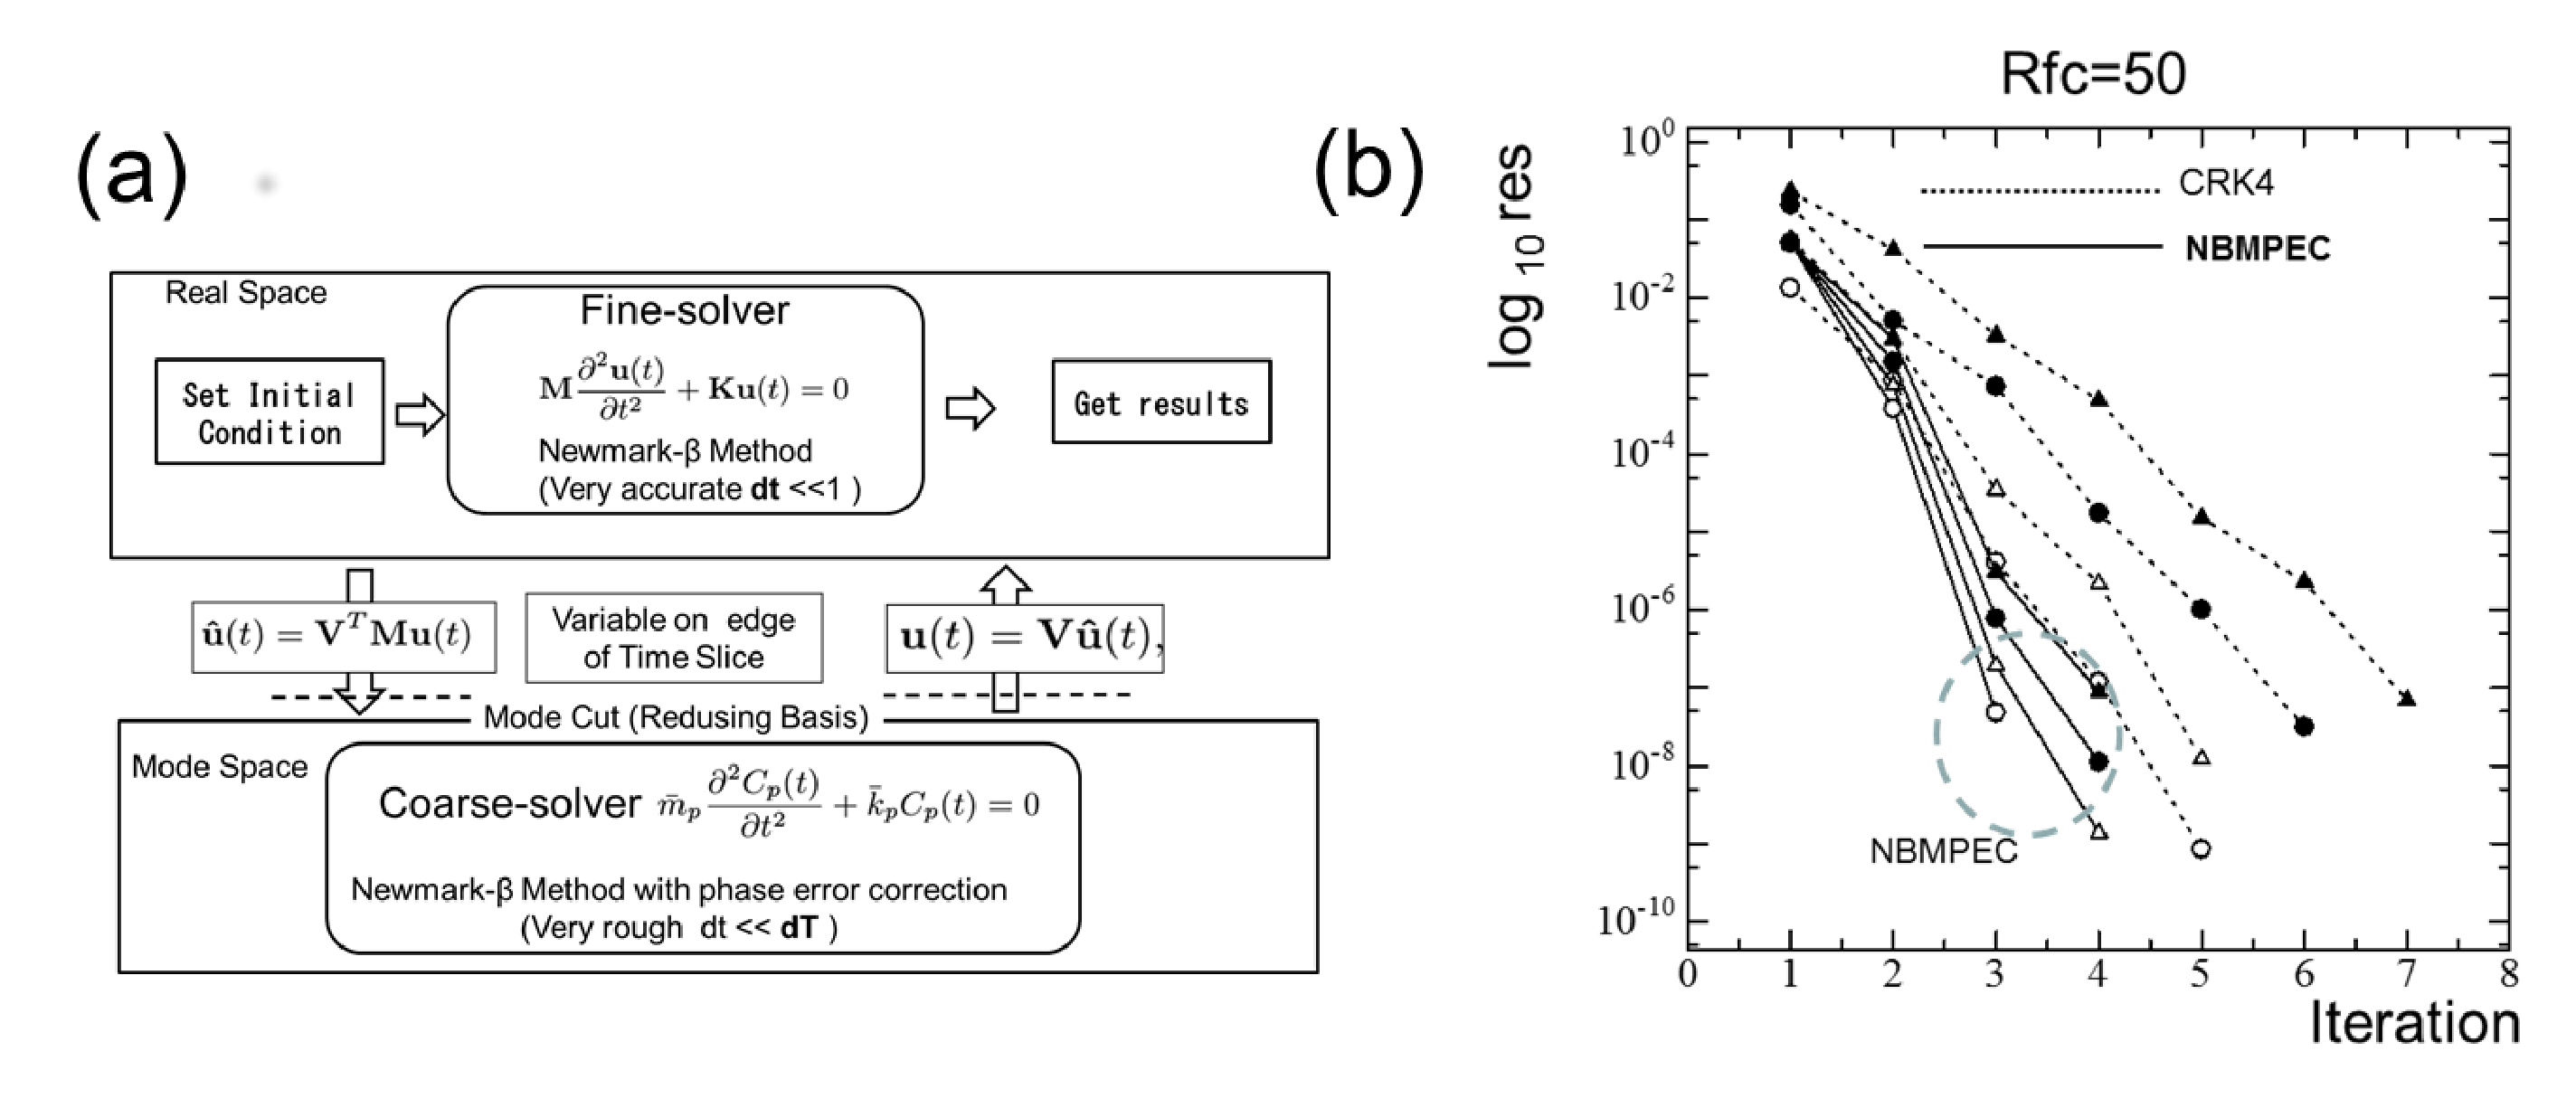
\includegraphics[scale=0.275]{research/ono/PinT-RBM.eps}
    \end{center}
    \caption{{\it PinT} methods: (a) {\it Parareal} process based on Reduced basis methods, (b) Convergence of {\it Parareal} method using {\it Newmark-$\beta$} method with phase error correction(NBMPEC) vs CRK4(Classical 4th-order Runge-Kutta method). Number of cycle = 100 ($\circ$), 1,000 ($\bigtriangleup$), 10,000 ($\bullet$), 100,000 ($\spadesuit$).}
    \label{fig:Methods}
\end{figure}

\subsection{Sparse Modeling}

Large-scale simulation usually needs several days, or even several months to be executed on current supercomputers. It is strongly desired by researchers to observe the visualization results of such kind of simulations in real time for analysis and adjustment of initial simulation parameters. However, due to the limitation of memory size, currently most of such kinds of simulation datasets are analysed as post processing such as visualization.
It is usually necessary to execute these large-scale simulations several times for selecting a set of good initial parameters for simulations and visualizations, and this leads to a time consuming process for scientists and engineers. In this research, we investigated a sparse modeling-based interactive {\it in-situ} visualization method, in order to assist the users to visualize the simulation results along with the running simulation. By analysing these visualization results in real-time, the users will be able to adjust the simulation parameters and restart the simulation  without the need for waiting to the conclusion of the entire simulation.  
As a result, it becomes possible to avoid the repetitive execution of the entire simulation just for the parameter selection process. The Proper Orthogonal Decomposition (POD) algorithm is used to design a sparse model for getting a good compression ratio for assisting the {\it in-situ} visualization.
We also investigated a data sharing approach between the simulation code and the compression code to obtain the best performance. The visualization framework shown in Figure~\localref{fig:HIVE} is employed for the rendering and interactive visualization. HIVE is a hardware independent parallel visualization system with a scalable rendering capability.

\section{Schedule and Future Plan}

The next big step for the \emph{HIVE} framework is its transition from the prototype stage to a solid and robust production-level system. During the early stage of the development, we have already held an initial presentation through the AICS Open Source Workshop Program to present an overview, and at the same time, to obtain a feedback from the potential users. In the next fiscal year, we are planning to take more advantage of this kind of AICS internal events, as well as other external events, not only for disseminating \emph{HIVE} system, but also to verify and discuss potential future enhancements based on the real-world requirements and needs. Focusing on the AICS internal demands, we are collaborating with some AICS teams involved in the computational science fields for utilizing their real simulation results. In this initial stage, we are using some datasets from the Computational Climate and Computational Fluid Dynamics(CFD) simulations, and have investigated some directions for further enhancements. We are planning to gradually enlarge this group of collaboration teams for aggregating new functionalities based on real world demands. The loosely coupled modular approach adopted by the HIVE system greatly facilitates the aggregation of new functionalities as native or third-party modules. Our initial priorities are: {\bf Fiber Surface}, {\bf FFV/C}\cite{2015:AVRTeam:FFVC}, {\bf PBVR}, and {\bf PIDX}. In the next fiscal year, we are planning to aggregate the large-scale {\bf PBVR} (Particle-Based Volume Rendering) functionality being developed under the Grant-in-Aid for Scientific Research (KAKENHI) in collaboration with Kyoto University and Kobe University. {\bf PIDX} is a data format for streaming based visualization developed by the University of Utah, which our team has a signed MOU (Memorandum of Understanding). In the next fiscal year, we will accept a graduate student from this university as a student trainee, in order to investigate the potential of this approach on the K computer environment and a future aggregation to \emph{HIVE} system.



%%% DO NOT EDIT BELOW

\section{Publications}

%\printbibliography[keyword=journal, heading=subbibliography, title={Journal Articles}, prefixnumbers={1-}, resetnumbers=true]
%\printbibliography[keyword=proceedings, heading=subbibliography, title={Conference Papers}, prefixnumbers={2-}, resetnumbers=true]
%\printbibliography[keyword=invited, heading=subbibliography, title={Invited Talks}, prefixnumbers={3-}, resetnumbers=true]
%\printbibliography[keyword=poster, heading=subbibliography, title={Posters and Presentations}, prefixnumbers={4-}, resetnumbers=true]
%\printbibliography[keyword=deliverable, heading=subbibliography, title={Patents and Deliverables}, prefixnumbers={5-}, resetnumbers=true]

\printbibliography[keyword=journal, heading=subbibliography, title={Journal Articles}, resetnumbers=true]
\printbibliography[keyword=proceedings, heading=subbibliography, title={Conference Papers}]
\printbibliography[keyword=invited, heading=subbibliography, title={Invited Talks}]
\printbibliography[keyword=poster, heading=subbibliography, title={Posters and Presentations}]
\printbibliography[keyword=deliverable, heading=subbibliography, title={Patents and Deliverables}]


\end{refsection}
